\documentclass[12pt,a4paper]{article}
\usepackage[T1]{fontenc}
\usepackage[utf8]{inputenc}
\usepackage{newtxtext,newtxmath}
\usepackage[a4paper,left=22mm,right=22mm,top=21mm,bottom=22mm]{geometry}
\usepackage{setspace}
\usepackage{amsmath}
\usepackage{graphicx}
\usepackage{booktabs}
\usepackage{float}
\usepackage[font=small,labelfont=bf]{caption}
\usepackage{microtype}
\usepackage{fancyhdr}
\usepackage{titlesec}
\usepackage[colorlinks=true,linkcolor=black,urlcolor=blue,breaklinks=true]{hyperref}
\usepackage{xurl}
\onehalfspacing
\setlength{\parindent}{0pt}
\setlength{\parskip}{5pt}
\setlength{\textfloatsep}{9pt}
\setlength{\intextsep}{8pt}
\renewcommand{\arraystretch}{1.13}
\titlespacing*{\section}{0pt}{0pt}{9pt}
\titlespacing*{\subsection}{0pt}{8pt}{5pt}
\titleformat{\section}{\large\bfseries}{\thesection}{.7em}{}
\titleformat{\subsection}{\normalsize\bfseries}{\thesubsection}{.7em}{}
\pagestyle{fancy}
\fancyhf{}
\renewcommand{\headrulewidth}{0pt}
\fancyfoot[L]{\footnotesize Saubach river water quality}
\fancyfoot[R]{\footnotesize\thepage}
\setcounter{tocdepth}{2}
\hypersetup{pdftitle={Seasonal and spatial patterns in Saubach river water quality},
pdfauthor={Mohamad Ghoroobi}}

\begin{document}
% Physical page 1: title. Edit your name and date here.
\thispagestyle{empty}
\vspace*{30mm}
\begin{center}
{\LARGE\bfseries Seasonal and spatial patterns\\[5pt]
in Saubach river water quality\par}
\vspace{12mm}
{\large Oxygen and nitrate across five river sections\par}
\vspace{25mm}
{\Large Mohamad Ghoroobi\par}
\vspace{8mm}
17 November 2026\par
\vspace{25mm}
Application Report\par
M.Sc.\ Data Science\par
TU Dortmund University\par
Summer Semester 2027\par
\vspace{18mm}
\small Project code, data and results:\par
\url{https://github.com/mohamadghoroobi/river-oxygene-and-nitrate-analyses}
\end{center}
\clearpage

% Physical page 2: contents only, generated from all section headings.
\begingroup
\singlespacing
\tableofcontents
\endgroup
\clearpage

% Pages 3--10: edit the separate section files.
\section{Introduction}
\subsection{Motivation and research questions}
Spatial and seasonal comparisons provide two complementary views of river water quality. A concentration measured near the headwaters may differ from one measured near the mouth; a seasonal average may also conceal a spatial pattern that changes through the year. Both sources of variation should therefore be considered when comparing measurements. This report examines oxygen and nitrate in the Saubach river, using the river name stipulated in the task.

The analysis addresses two questions. First, do spring and autumn differ in mean oxygen or nitrate concentration? Second, do mean concentrations differ among the five river sections, and which section pairs differ? All concentrations and estimated differences are expressed in milligrams per liter (mg/L). The seasonal comparison averages equally over sections, while each spatial comparison averages equally over seasons.

\subsection{Approach and principal findings}
The supplied dataset contains 900 observations in a balanced design: five river sections, four seasons, and 45 observations in each section--season combination. Descriptive summaries and figures show the location, spread, and shape of the concentrations. A full factorial model retains the section-by-season interaction. Heteroskedasticity-robust contrasts then address the research questions. Holm adjustment is applied across both analytes to limit the probability of at least one false rejection, using the specified significance level $\alpha=0.075$.

The main findings are as follows. Mean nitrate is higher in spring than autumn by $0.871$ mg/L, and every section pair differs for nitrate after adjustment. Mean oxygen is higher in spring by $0.152$ mg/L, but that comparison does not reject after adjustment. Seven oxygen section pairs differ when averaged over seasons. Oxygen also shows a section-by-season interaction, so its spatial differences should not be described as constant throughout the year.

These conclusions depend on the assumed independence of the observations. The data do not provide sampling dates or repeated-site identifiers with which to verify this assumption. The report quantifies the observed patterns without attributing them to an unmeasured environmental cause.

Section~\ref{sec:data} describes the data and estimands. Section~\ref{sec:methods} defines and justifies the methods. Section~\ref{sec:evaluation} presents the descriptive and inferential results. Section~\ref{sec:summary} answers the questions and discusses limitations.

\clearpage
\section{Data and problem definition}\label{sec:data}
\subsection{Source, measurements and design}
The dataset \texttt{waterquality.csv} was supplied by TU Dortmund University for the summer-semester 2027 M.Sc.\ Data Science application task. It was downloaded on 17 November 2026 from the URL given in the application brief. The original CSV, source URL, download date, file size, and SHA-256 checksum are retained in the project repository. ``Saubach'' is the name assumed for this analysis as requested; the CSV itself does not identify the river.

The five sections are ordered from headwaters to mouth: A1 (headwaters), A2 (upper course), A3 (middle course), A4 (lower course), and A5 (mouth). Each section contains 180 rows: 45 in each of spring, summer, autumn, and winter. Thus, every season contains 225 observations. Each row contains both an oxygen and a nitrate measurement. Table~\ref{tab:variables} summarizes the variables and their role.

\begin{table}[H]
\centering\small\singlespacing
\begin{tabular}{lll}
\toprule
Variable & Meaning & Statistical role \\
\midrule
\texttt{ID} & Row identifier & Validation only \\
\texttt{river\_section} & Five ordered sections & Categorical predictor \\
\texttt{saison} & Four seasons & Categorical predictor \\
\texttt{oxygen\_mgL} & Oxygen, mg/L & Quantitative outcome \\
\texttt{nitrate\_mgL} & Nitrate, mg/L & Quantitative outcome \\
\bottomrule
\end{tabular}
\caption{Variables in the original semicolon-separated CSV.}\label{tab:variables}
\end{table}

\subsection{Validation and information limits}
All 900 observations were retained. Validation found no missing values, duplicate IDs, duplicate complete rows, negative concentrations, or nonfinite values. The expected 45 observations were present in every section--season cell. No imputation or outcome-based exclusion was performed.

Section is modeled categorically because no distances between sections are supplied. Season is also categorical. The ID is neither a predictor nor evidence that measurements are temporally ordered or paired. Oxygen and nitrate appear in the same rows, but the two analytes are modeled separately; multiplicity correction includes both outcomes.

The file does not give sampling dates, repeated-site identifiers, collection methods, or measurement protocols. Independent errors are therefore an explicit assumption. Without additional metadata, neither representativeness for other rivers or years nor a causal explanation of the observed differences can be established.

\clearpage
\section{Statistical methods}\label{sec:methods}
\subsection{Full factorial model and its justification}
For each analyte separately, let $Y_{ijk}$ denote observation $k$ in section $i$ and season $j$, where $i=1,\ldots,5$, $j=1,\ldots,4$, and $k=1,\ldots,45$. The full factorial model is expressed in cell-means form:
\begin{equation}
Y_{ijk}=\mu_{ij}+\varepsilon_{ijk},\qquad
E(\varepsilon_{ijk})=0,\quad
\operatorname{Var}(\varepsilon_{ijk})=\sigma_{ij}^{2}.
\end{equation}
This model assigns each section--season combination its own mean. It retains the interaction rather than assuming identical spatial differences in every season, and permits unequal variances across the 20 cells.

In matrix form, $\mathbf Y=X\boldsymbol\beta+\boldsymbol\varepsilon$, where $X$ has one indicator column per cell. The least-squares estimate is
\begin{equation}
\widehat{\boldsymbol\beta}=(X^\top X)^{-1}X^\top\mathbf Y.
\end{equation}
The disjoint indicator columns make each coefficient its sample cell mean. There are $900-20=880$ residual degrees of freedom.

\subsection{Contrasts and scientific interpretation}
The spring--autumn and section-pair estimands are
\begin{align}
\Delta&=\frac15\sum_{i=1}^{5}
  (\mu_{i,\mathrm{spring}}-\mu_{i,\mathrm{autumn}}),\\
D_{ab}&=\frac14\sum_{j=1}^{4}(\mu_{aj}-\mu_{bj}),\quad a<b.
\end{align}
Positive $\Delta$ means higher spring concentration; positive $D_{ab}$ means higher concentration in section $a$. The weights give sections and seasons equal representation. Because the data are balanced, these estimates equal the corresponding pooled mean differences. The underlying cell differences need not be constant.

\subsection{Heteroskedasticity-robust covariance}
With residual $e_r$ and leverage $h_r$, the HC3 estimator is
\begin{equation}
\widehat V=(X^\top X)^{-1}X^\top
 \operatorname{diag}\!\left\{\frac{e_r^2}{(1-h_r)^2}\right\}
 X(X^\top X)^{-1}.
\end{equation}
Here $h_r=1/45$. A cell's diagonal element simplifies to $s_{ij}^2/44$, using its residual sum of squares $44s_{ij}^2$ and inverse design factors $1/45$. Direct cell calculations verify this identity. HC3 does not correct spatial or temporal dependence.

\clearpage
\subsection{Hypotheses and test statistics}
For each outcome, the seasonal null is $H_0:\Delta=0$ against $H_1:\Delta\ne0$. The omnibus section null is equality of all five seasonal-average section means, represented by four independent contrasts. Each of the ten section-pair nulls is $H_0:D_{ab}=0$. A further 12-contrast test checks absence of interaction:
\begin{equation}
(\mu_{ij}-\mu_{i1})-(\mu_{1j}-\mu_{11})=0,
\qquad i>1,\ j>1.
\end{equation}
For a $q$-row contrast matrix $L$, the Wald statistic is
\begin{equation}
W=(L\widehat{\boldsymbol\beta})^\top
 (L\widehat V L^\top)^{-1}
 (L\widehat{\boldsymbol\beta})\ \dot\sim\ \chi_q^2.
\end{equation}
For a scalar contrast $c$, the signed statistic is
$z=c^\top\widehat{\boldsymbol\beta}/\sqrt{c^\top\widehat Vc}$ and $W=z^2$. Two-sided $p$-values use a standard normal reference for $z$; joint tests use the indicated chi-square reference. These are asymptotic approximations, not exact finite-sample tests. Repeated observations in each cell support approximation of the cell means, conditional on independent sampling and finite variances.

\subsection{Multiplicity and interval coverage}
The significance level is $\alpha=0.075$. One family contains all 26 tests: two seasonal, two section omnibus, twenty section pairs, and two interactions. For ordered raw $p$-values $p_{(1)},\ldots,p_{(26)}$, Holm-adjusted values are
\begin{equation}
p^{\mathrm{adj}}_{(k)}=
\min\left\{1,\max_{1\le r\le k}(26-r+1)p_{(r)}\right\}.
\end{equation}
Reject if $p^{\mathrm{adj}}\le0.075$. To see the familywise protection, suppose $m_0$ nulls are true. At the first true rejection, the threshold is no greater than $\alpha/m_0$. The union bound over the $m_0$ true nulls therefore bounds any false rejection by $\alpha$, provided their individual $p$-values are valid. Here that validity is approximate because Wald references are asymptotic.

Pointwise $92.5\%$ intervals are estimate $\pm z_{0.9625}$ times standard error, with $z_{0.9625}\approx1.7805$. They are not simultaneous intervals. A pointwise interval may exclude zero even when the globally adjusted test does not reject.

\subsection{Descriptive summaries and model checks}
Descriptive summaries use means, sample SDs, medians, quartiles, and ranges. Boxplots show the median and the interval from $Q_1$ to $Q_3$; whiskers reach the furthest observations within $1.5(Q_3-Q_1)$ of the box. Other observations are displayed and retained. Quartiles use linear interpolation. Residual-versus-fitted and normal Q--Q plots inspect spread and shape. The HC2 sensitivity estimator replaces $(1-h_r)^2$ by $1-h_r$ in HC3; here it scales the covariance by $44/45$.

\clearpage
\section{Evaluation}\label{sec:evaluation}
\subsection{Descriptive seasonal analysis}
Table~\ref{tab:seasonal} describes the seasonal concentrations. Oxygen has its lowest mean in summer (7.040 mg/L) and its highest mean in winter (9.935 mg/L). Nitrate has its highest mean in summer (10.342 mg/L) and its lowest mean in winter (7.198 mg/L). Each season contains the same number of measurements from each river section.

\begin{table}[H]
\centering\small\singlespacing
\begin{tabular}{lrrr}
\toprule
Season & $n$ & Oxygen: mean (SD) & Nitrate: mean (SD) \\
\midrule
Spring & 225 & 9.531 (0.857) & 9.289 (2.591) \\
Summer & 225 & 7.040 (0.930) & 10.342 (2.744) \\
Autumn & 225 & 9.379 (0.888) & 8.418 (2.752) \\
Winter & 225 & 9.935 (0.779) & 7.198 (2.442) \\
\bottomrule
\end{tabular}

\caption{Seasonal mean and sample SD in mg/L, pooled over five sections.}\label{tab:seasonal}
\end{table}

Figure~\ref{fig:seasonal} shows the distributions. Spring and autumn oxygen overlap substantially. Their nitrate distributions also overlap, despite a larger difference in their means. Distributional overlap alone does not decide a test of mean differences; the inferential analysis evaluates uncertainty and multiplicity separately.

\begin{figure}[H]
\centering
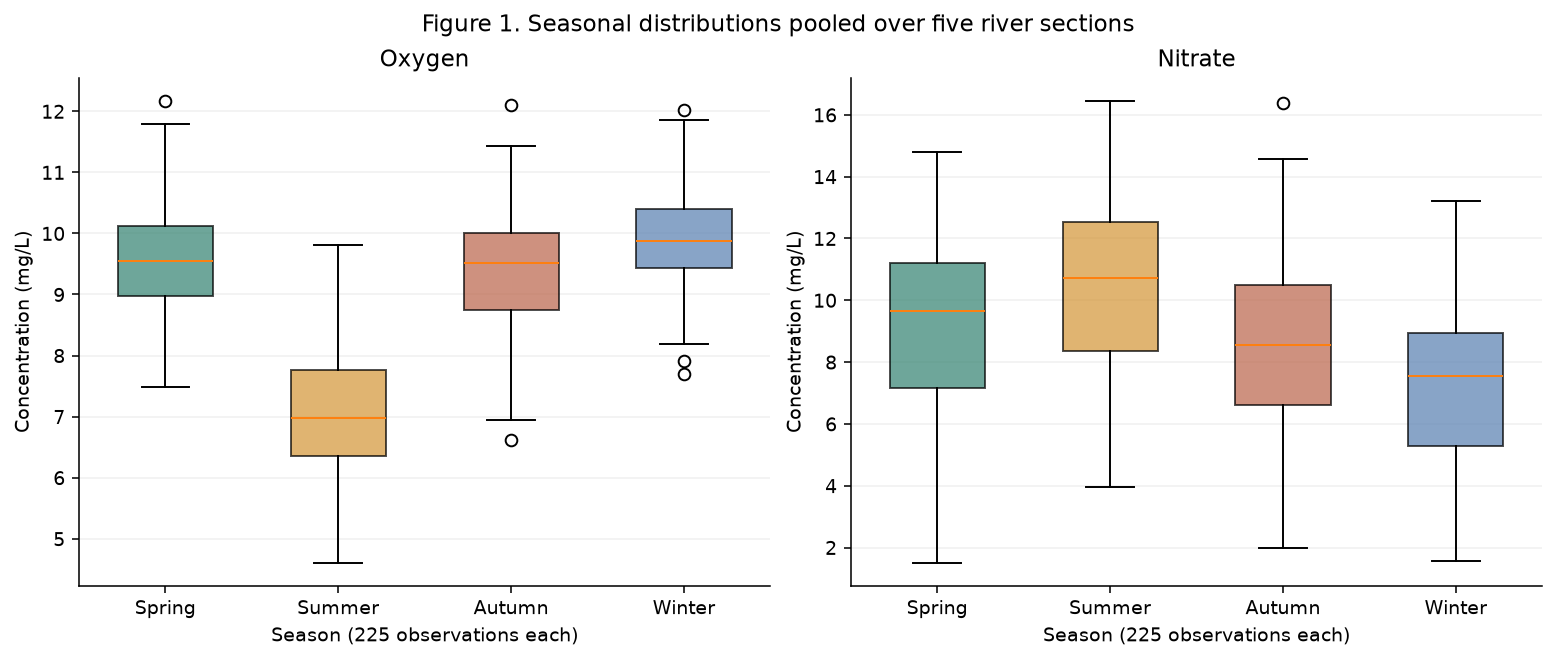
\includegraphics[width=\linewidth]{figures/seasonal_distributions.png}
\caption{Seasonal distributions, with 225 observations per season. Boxes mark the quartiles and median. Whiskers use the 1.5-IQR rule; points beyond them are retained observations.}\label{fig:seasonal}
\end{figure}

Spring oxygen has median 9.550 mg/L and IQR 1.153 mg/L; autumn oxygen has median 9.514 mg/L and IQR 1.265 mg/L. Spring nitrate has median 9.652 mg/L and IQR 4.039 mg/L; autumn nitrate has median 8.568 mg/L and IQR 3.883 mg/L. These location and dispersion summaries complement the means and SDs in Table~\ref{tab:seasonal}.

\clearpage
\subsection{Descriptive spatial analysis}
Table~\ref{tab:sections} summarizes concentrations across sections, averaging the four seasons equally. Mean nitrate increases from 5.350 mg/L at the headwaters to 11.467 mg/L at the mouth. Mean oxygen ranges from 8.694 mg/L in the lower course to 9.231 mg/L at the headwaters. Its pooled spatial profile is not monotonic: the mouth has a higher oxygen mean than the lower course.

\begin{table}[H]
\centering\small\singlespacing
\begin{tabular}{lrrr}
\toprule
Section & $n$ & Oxygen: mean (SD) & Nitrate: mean (SD) \\
\midrule
A1: Headwaters & 180 & 9.231 (1.230) & 5.350 (1.708) \\
A2: Upper course & 180 & 9.005 (1.280) & 7.343 (1.789) \\
A3: Middle course & 180 & 8.990 (1.409) & 9.328 (1.809) \\
A4: Lower course & 180 & 8.694 (1.465) & 10.570 (1.858) \\
A5: Mouth & 180 & 8.936 (1.665) & 11.467 (1.985) \\
\bottomrule
\end{tabular}

\caption{Section means and sample SDs in mg/L, pooled over four seasons.}\label{tab:sections}
\end{table}

Figure~\ref{fig:spatial} separates the section profiles by season. Nitrate rises downstream in all four seasons. Summer oxygen decreases toward the mouth, whereas winter oxygen varies relatively little between sections. Autumn oxygen is lower in A4 and higher again in A5. Thus, the spatial oxygen profiles are not parallel across seasons.

\begin{figure}[H]
\centering
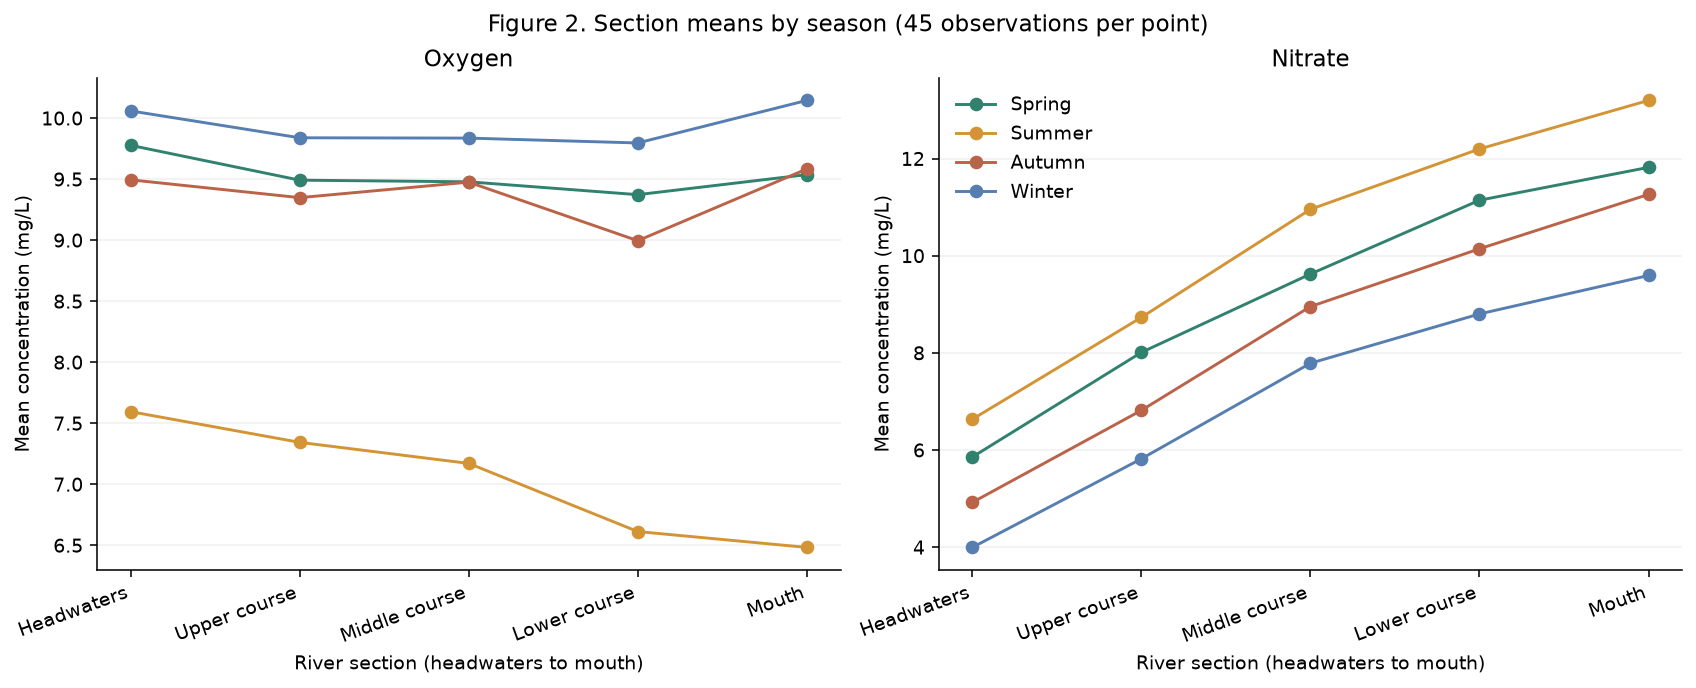
\includegraphics[width=\linewidth]{figures/section_season_means.png}
\caption{Section means by season; each point represents 45 observations. Connecting lines link ordered categories and do not fit a continuous spatial model.}\label{fig:spatial}
\end{figure}

Pooled section SDs include both seasonal variation and within-season variability. For this reason, they are not substituted for within-cell variances in the factorial contrasts. The inferential model estimates the 20 cell means and uses their residual variability. This preserves the observed balance while retaining different spatial patterns in different seasons.

\clearpage
\subsection{Seasonal tests and section comparisons}
Table~\ref{tab:season-tests} answers the spring--autumn question. Nitrate rejects after Holm adjustment; oxygen does not. The oxygen pointwise interval excludes zero, but its adjusted $p$-value exceeds 0.075 because the interval does not correct for the 26 comparisons. Failure to reject does not establish equivalence.

\begin{table}[H]
\centering\footnotesize\singlespacing
\begin{tabular}{lrrrr}
\toprule
Outcome & Difference & 92.5\% pointwise CI & Raw $p$ & Holm $p$ \\
\midrule
Oxygen & 0.152 & [0.005, 0.298] & 0.0647 & 0.3236 \\
Nitrate & 0.871 & [0.618, 1.123] & $8.11\times10^{-10}$ & $1.22\times10^{-8}$ \\
\bottomrule
\end{tabular}

\caption{Spring minus autumn, averaged over sections. Differences and pointwise intervals are in mg/L.}\label{tab:season-tests}
\end{table}

Table~\ref{tab:omnibus} shows section differences for both analytes and an interaction for oxygen. The nitrate interaction does not reject. All pairwise results are given in Table~\ref{tab:pairs}.

\begin{table}[H]
\centering\footnotesize\singlespacing
\begin{tabular}{lrrr}
\toprule
Outcome / null hypothesis & $W$ & df & Holm $p$ \\
\midrule
Oxygen / equal section means & 42.70 & 4 & $1.55\times10^{-7}$ \\
Oxygen / no interaction & 48.30 & 12 & $3.33\times10^{-5}$ \\
Nitrate / equal section means & 2112.21 & 4 & $<10^{-99}$ \\
Nitrate / no interaction & 10.53 & 12 & 1.0000 \\
\bottomrule
\end{tabular}

\caption{Joint robust Wald tests with chi-square reference distributions.}\label{tab:omnibus}
\end{table}

\begin{table}[H]
\centering\footnotesize\singlespacing
\begin{tabular}{lrrrr}
\toprule
Pair & $D_{ab}$: oxygen & Holm $p$ & $D_{ab}$: nitrate & Holm $p$ \\
\midrule
A1--A2 & 0.226 & 0.0554 & -1.993 & $4.06\times10^{-39}$ \\
A1--A3 & 0.241 & 0.0554 & -3.978 & $<10^{-99}$ \\
A1--A4 & 0.537 & $1.42\times10^{-9}$ & -5.220 & $<10^{-99}$ \\
A1--A5 & 0.294 & 0.0059 & -6.116 & $<10^{-99}$ \\
A2--A3 & 0.015 & 1.0000 & -1.985 & $1.21\times10^{-38}$ \\
A2--A4 & 0.311 & 0.0035 & -3.227 & $<10^{-99}$ \\
A2--A5 & 0.069 & 1.0000 & -4.124 & $<10^{-99}$ \\
A3--A4 & 0.296 & 0.0117 & -1.242 & $1.14\times10^{-15}$ \\
A3--A5 & 0.053 & 1.0000 & -2.138 & $2.03\times10^{-41}$ \\
A4--A5 & -0.243 & 0.0421 & -0.897 & $9.19\times10^{-8}$ \\
\bottomrule
\end{tabular}

\caption{Section contrasts: first section minus second, averaged over seasons, in mg/L. All three test tables share one 26-test Holm adjustment. Very small adjusted $p$-values are shown as $<10^{-99}$.}\label{tab:pairs}
\end{table}

All ten nitrate pairs reject at 0.075. Seven oxygen pairs reject: A1--A2, A1--A3, A1--A4, A1--A5, A2--A4, A3--A4, and A4--A5. A2--A3, A2--A5, and A3--A5 do not reject. These statements concern seasonal-average section means.

\clearpage
\section{Summary and discussion}\label{sec:summary}
\subsection{Answers to the research questions}
The analysis compared oxygen and nitrate concentrations in the Saubach river across five sections and four seasons. All 900 observations were retained in a balanced design. Tests used a full factorial model, HC3 covariance, and Holm adjustment across 26 hypotheses at $\alpha=0.075$.

For spring versus autumn, mean nitrate is higher in spring by 0.871 mg/L, averaged equally over the five sections (adjusted $p=1.22\times10^{-8}$). Mean oxygen is higher in spring by 0.152 mg/L, but its adjusted $p=0.324$ does not provide sufficient evidence of a difference. This non-rejection does not demonstrate equal concentrations.

Both analytes show differences between section means averaged over seasons. Every nitrate pair differs, with progressively higher means downstream. For oxygen, A1 differs from all four other sections, and A4 also differs from A2, A3, and A5. The oxygen interaction shows that its spatial pattern depends on season, so these seven pairwise differences are averages rather than a common pattern throughout the year.

\subsection{Diagnostic evidence and limitations}
Within-cell SDs range from 0.648 to 1.090 mg/L for oxygen and 1.181 to 1.746 mg/L for nitrate, supporting a covariance estimator that permits different variances. Residual Q--Q plots show approximately linear overall patterns, with some tail departures. The residual plots and full diagnostics are supplied with the analysis code. Replacing HC3 with HC2 leaves all 26 adjusted decisions unchanged. Direct cell calculations also reproduce the estimated means and HC3 covariance to numerical precision.

The main limitation is the unknown sampling design. The CSV does not identify sampling dates or repeated sites. If measurements are correlated in time or space, the independent-error covariance may understate or otherwise misrepresent uncertainty; HC3 does not solve that problem. The significance conclusions are therefore conditional on independent sampling and the accuracy of asymptotic approximation.

The downstream nitrate gradient and low summer oxygen identify patterns for further investigation. The data do not establish their causes or whether concentrations imply environmental harm. Additional sampling metadata and contextual measurements would be needed before considering a dependence model, explanatory mechanisms, or applicable environmental thresholds.

\subsection{Project materials}
The original dataset, download provenance, executable scripts, numerical results, figures, and editable report sources are available in the project repository:\par
\small\url{https://github.com/mohamadghoroobi/river-oxygene-and-nitrate-analyses}

\end{document}
